\section{Un Réseau}

\paragraph{Réseaux naturels, n\oe{}uds, liens}

\paragraph{} Bien que le terme de réseau ne se soit largement démocratisé que depuis quelques dizaines d'années, il tire ses
racines plus anciennes du latin \emph{resel} qui signifiait \emph{le filet}. On retrouve ici la caractéristique
principale du réseau : ce sont des \emph{n\oe{}uds liés} entre eux selon un \emph{schéma}. Les réseaux existent en
premier lieu sous forme naturelle, on pense alors aux cours d'eau et à leurs conjonctions, aux mouvements de troupeaux,
aux racines des arbres. Nous remarquons que les constructions humaines suivent également des réseaux : le réseau routier
avec les villes comme n\oe{}uds, le réseau ferré et les gares, le réseau électrique et les centrales...

\paragraph{} Toute création regroupant des n\oe{}uds avec des relations entre ces n\oe{}uds peut être qualifiée de "Réseau". En sciences,
la discipline qui s'occupe d'étudier les réseaux, et qui regroupe mathématique et informatique, s'appelle
la \emph{Théorie des Graphes}. Lorsque toute relation entre deux n\oe{}uds d'un graphe est symétrique, c'est à dire qu'elle va
dans un sens et dans l'autre, nous parlons de graphes \emph{non orientés}. Ce n'est par exemple pas le cas pour le
réseau routier qui est un graphe \emph{orienté}, car il possède des rues \emph{à sens unique}.

\begin{figure}[h]
    \centering
    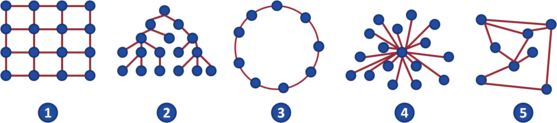
\includegraphics[width=400px]{chapters/02/images/reseaux.png}
    \caption{\label{Réseaux, graphes} Différentes formes de graphes}
\end{figure}

\paragraph{} On peut retrouver naturellement certaines de ces constructions. Le réseau hiérarchique (2) existe
au sein des sociétés, des gouvernements et des groupes d'Hommes en général. Il décrit généralement une structure
de contrôle par le haut, où le n\oe{}ud le plus haut est dit \emph{parent} des n\oe{}uds juste en dessous, et ainsi de suite.
Ainsi le pouvoir se concentre sur le haut du réseau et peut facilement être transmis verticalement, mais pas de 
manière transverse.

\paragraph{} On retrouve également le réseau centralisé (4) dans les organisations humaines par exemple,
où il traduit simplement la référence directe à un pouvoir supérieur. Les n\oe{}uds n'ont pas besoin de connaître
l'existence d'autres n\oe{}uds car ils se réfèrent directement à une unité centrale qui sera \emph{décisionnaire}.
Souvent, les réseaux centralisés forment entre eux d'autres réseaux centralisés plus importants afin de reléguer
toute les \emph{micro-décisions} à une entité centrale supérieure qui sera en charge, à partir de ces informations,
de calculer une \emph{macro-décision}. On retrouve ici la notion de \emph{couches}, qui nous servira dans l'étude
de réseaux plus complexes.

\paragraph{} Par opposition à la centralisation, le réseau décentralisé (5) est à l'image d'un système décisionnaire au
sein duquel chaque participant peut faire entendre sa voix. Il n'est pas nécessaire pour un participant d'avoir connaissance
de l'ensemble des membres du réseau, car l'information est transmise de n\oe{}ud en n\oe{}ud, à travers le maillage.
Cela permet notamment de mettre en place des réseaux beaucoup plus résilients : si l'un des n\oe{}uds est déconnecté,
le réseau peut continuer de fonctionner.


\paragraph{Types de réseaux}

\paragraph{} En informatique, lorsque plusieurs machines sont connectées entre elles, le plus souvent par des câbles, on
parle alors de \emph{réseau}. Afin de comprendre pourquoi certaines topologies de réseaux existent, nous allons introduire 
deux types de réseaux bien connus : \emph{le LAN et le WAN}.

\paragraph{} Le LAN, ou Local Area Network, se limite à un espace géographique déterminé. On peut prendre
par exemple le contenu d'une salle, un étage, un immeuble. Ainsi les réseaux d'une école, d'un
hopital, d'une gare, d'un aéroport, sont des LANs. Pour parler de transmission sans fil, ou
Wi-Fi, on utilise aussi le terme \emph{WLAN}, pour Wireless LAN. Les points d'accès Wi-Fi, qui se
sont démultipliés dans les cafés, restaurants, lieux d'attente, aéroports à travers le monde
sont des exemples de WLAN.

\paragraph{} Le WAN signifie Wide Area Network, ou réseau étendu. Il est en fait formé par
l'association de plusieurs LANs. On retrouve ici la notion de réseaux \emph{composés}. Des LANs,
reliés entre eux, forment un réseau à part entière, qui peut lui même se connecter à d'autres
LANs ou WANs.


\paragraph{Réseau nominal} 

\paragraph{} Aujourd'hui, les réseaux informatiques que nous utilisons au quotidien sont composés
de l'exacte manière que nous venons de présenter : une multitude de - plus ou moins - petits LANs, et un empilement
par couches successives de WANs dont le dernier, \emph{internet}, les met tous en relation. Il est inutile de divaguer
sur la mise en place d'un \emph{réseau universel}, car celui-ci est déjà en place. Omniprésent, nous l'utilisons au
quotidien.

\paragraph{} Il serait normalement nécessaire de prendre en considération les aspects liés à la gouvernance de ce réseau 
mondial, entre intérêts des États et des opérateurs de télécommunication. Mais nécessaire uniquement s'il était question
de \emph{prendre contrôle} du réseau ; hors ce n'est pas de cela qu'il s'agit. Car contrôler le réseau implique des 
responsabilités, tandis qu'en tirer parti n'entraîne - virtuellement - que des avantages.

\paragraph{} Mais quand on parle de réseau, il est important de ne pas s'arrêter qu'au sens \emph{physique}, matériel du
terme. Car sur un même réseau physique peuvent cohabiter une multitude de réseaux logiques - \emph{logiciels}. C'est cet
aspect des réseaux qui va nous intéresser plus particulièrement, car si un réseau physique est un \emph{moyen}, un réseau
logique a une \emph{fin}.

\paragraph{} Sur ce réseau nominal vont être mis en place une multitude de réseaux logiques fournissant des services à
leurs utilisateurs. Cependant, la nature \emph{centralisée} de ces réseaux rend aisé la mise en place d'une censure de
l'information, quelle qu'elle soit. De même, l'utilisateur n'a d'autre choix que de faire \emph{confiance} à l'entité
lui fournissant un service en ce qui concerne les données qu'elle transmet.

\paragraph{} Et bien souvent, entre l'utilisateur et le service, on retrouve un acteur incontournable : le moteur de
recherche. Le rôle de ce service est double : il va dans un premier temps \emph{indexer} le plus de contenus possible
accessible sur internet, et dans un second temps permettre à un utilisateur d'effectuer une recherche par mots clés 
pour lui renvoyer les contenus jugés les plus appropriés. Certains moteurs, plus spécifiques, utilisent leur base
d'indexation pour fournir non plus un \emph{contenu} brut mais un ensemble de \emph{connaissances} liées à la requête
de l'utilisateur \cite{Internet2}.

\paragraph{} Le rôle à jouer des moteurs de recherche dans l'écosystème technologique actuel est colossal : ils peuvent
presque être considérés comme la "porte" d'internet, permettant de trouver un contenu approprié à notre besoin en quelques
instants. Mais encore une fois ce service est à double tranchant, car les résultats renvoyés par le moteur sont fonction
du contenu de sa base d'indexation. De fait Tim Bray, ancien employé de Google travaillant aujourd'hui chez Amazon Web Services,
a remarqué que certains vieux articles de blogs étaient devenus, début 2018, totalement introuvables en utilisant le plus
important moteur de recherche mondial... alors que les résultats ressortaient bien sur d'autres services et que les pages 
étaient évidemment toujours accessibles \cite{Internet3}.

\paragraph{} Il ne s'agit là que d'un exemple, mais il met en exergue le déséquilibre de la balance des pouvoirs dans un 
modèle centralisé, dans lequel les n\oe{}ud périphériques (les utilisateurs) sont à la merci du n\oe{}ud central (fournissant
le service).


\paragraph{Réseaux parallèles}

\paragraph{} C'est ce constat qui a servi de base au développement de réseaux dits \emph{parallèles}.

\paragraph{TODO} Réseaux parallèles. Verra-t-on un jour la disparition des réseaux parallèles
(TOR, blockchains, ...) ? Ces technologies \emph{disruptives} seront-elles un jour vouées
à disparaitre ou au contraire à se développer avec d'autant plus d'ardeur ? Peut-on alors
parler d'une neutralisation du Réseau par le réseau ?

\paragraph{TODO} Le web, le 'dark web' (TOR), un seul et même réseau - le principe du rencensement. 
Les dérives, comment contrôler ? Peut-on contrôler, doit-on contrôler ? Exemple de la neutralité du net.

\paragraph{TODO} La révolution des réseaux parallèles : les blockchains. Qu'est-ce ? L'évolution des premiers jours et 
la Hype récente. L'évolution du cours du BTC comme exemple de l'engouement. Ethereum : la révolution des DApps.
Quel avenir pour les réseaux parallèles ? Neutralisation du réseau par le réseau. Transparence et anonymité.


\paragraph{Réseau... universel ?}

\paragraph{} Ainsi, puisque notre vecteur d'échange est déjà en place, 

\paragraph{TODO} "Idéal" de la mise en place d'un Réseau universel, omniprésent
et omniscient. Un tel système global impliquerait la mise en place d'un système hautement
distribué, voire \emph{"participatif"}.

\paragraph{TODO} Qu'est-ce qu'un réseau 'universel' ? Quels sont ses avantages ? Ses inconvénients ?
Qu'implique techniquement sa mise en place ? Est-ce réalisable aujourd'hui ? Qu'est-ce qu'un réseau distribué ? 